	% Welcome! This is the unofficial University of Udine beamer template.

% We defined four theme colors: UniBrown, UniBlue, UniGold
% and UniOrange. For example, to write some uniud-brownish
% text, just use: \textcolor{UniBrown}{Hello!}

\documentclass[usenames,dvipsnames, 10pt]{beamer}
\usepackage[utf8]{inputenc}
\usepackage{algorithm2e}
\usepackage{verbatim}
\usetheme{uniud}
%\bibliography{bib}
%%% Bibliography
%\usepackage[style=authoryear,backend=biber]{biblatex}
%\addbibresource{bib.bib}
\usepackage{tikz}
\usetikzlibrary{patterns,snakes}
%\DeclareNameAlias{author}{first-last}

%%% Suppress biblatex annoying warning
\usepackage{silence}
\WarningFilter{biblatex}{Patching footnotes failed}

%%% Some useful commands
% pdf-friendly newline in links
\newcommand{\pdfnewline}{\texorpdfstring{\newline}{ }} 
% Fill the vertical space in a slide (to put text at the bottom)
\newcommand{\framefill}{\vskip0pt plus 1filll}
\newcommand{\bigCI}{\mathrel{\text{\scalebox{1.07}{$\perp\mkern-10mu\perp$}}}}
\newcommand\asto{\mathrel{\stackrel{\makebox[0pt]{\mbox{\normalfont\tiny a.s.}}}{\to}}}


\newcommand{\independent}{\mbox{${}\perp\mkern-11mu\perp{}$}}
\newcommand{\notindependent}{\mbox{${}\not\!\perp\mkern-11mu\perp{}$}}
\newcommand{\iid}{\overset{\text{iid}}{\sim}}

\newcommand{\R}{\mathbb{R}}
\newcommand{\E}{\mathbb{E}}
%\newcommand{\C}{\mathbb{C}}

\newcommand{\y}{\mathbf{y}}
\newcommand{\uu}{\mathbf{u}}
\newcommand{\z}{\mathbf{z}}
\newcommand{\vv}{\mathbf{v}}
\newcommand{\w}{\mathbf{w}}
\newcommand{\x}{\mathbf{x}}

\newcommand{\Hyp}{\mathcal{H}}
\newcommand{\Myp}{\mathcal{M}}
\newcommand{\Ayp}{\mathcal{A}}

\newcommand{\Yspace}{\mathcal{Y}}
\newcommand{\Xspace}{\mathcal{X}}


\newcommand{\RR}{\mathbb{R}}

\title[Online Learning with Relative Lipschitz Losses]{‌\vspace{0.5cm}\\
Online Learning with Relative Lipschitz Losses}
\author[Behrad Moniri]{
  Behrad Moniri
  \pdfnewline
  \texttt{bemoniri@ee.sharif.edu}
}
\institute{\small{EE Department, Sharif University of Technology}}
\date{January 7, 2021}
\begin{document}

\begin{frame}
\titlepage
\end{frame}


\begin{frame}
	\frametitle{Outline}
	\tableofcontents
\end{frame}

\section{Online Convex Optimization}
\framecard{\LARGE Online Convex Optimization}

\begin{frame}
	\frametitle{Online Convex Optimization: Introduction}	
	\begin{algorithm*}[H]
		\SetAlgoLined
		\TitleOfAlgo{Online Convex Optimization}
		\KwIn{A convex set $S$.}
		\For{$t = 1, \dots, T$}{
			Predicts a vector $\w_t \in S$.\\
			Recieve a convex loss function $l_t: S \to \mathbb{R}$. \\
			Suffer loss $l_t(\w_t)$.
		}		
	\end{algorithm*}
	\begin{itemize}	
		\pause	
		\item Define a notion of {\color{brown} regret}:
		\vspace{-0.3cm}
		\begin{equation*}
		\mathrm{Regret}_T(\uu) = \sum_{t = 1}^{T} f_t(\w_t) - \sum_{t = 1}^{T} f_t(\uu).
		\end{equation*}
		\pause
		\vspace{-0.3cm}
		\item Our goal is to minimize:
		\vspace{-0.3cm}
		\begin{equation*}
		\max_{\uu\in S}\Big( \mathrm{Regret}_T(\uu)\Big)
		\end{equation*}		
	\end{itemize}			
\end{frame}


\begin{frame}
	\frametitle{Online Convex Optimization: Applications}		
	\begin{itemize}		
		\item \textbf{Convex Optimization:} Adversary plays a fixed $f$.
		
		$$f\big(\frac{1}{T}\sum_{t = 1}^{T}\w_t\big) - f(\w*) \leq \frac{1}{T}\sum_{t=1}^{T} f(\w_t) - \frac{1}{T}\sum_{t=1}^{T} f(\w^*) = \frac{\mathrm{Regret}_T(\w^*)}{T}$$
		\pause
		\item \textbf{Online Linear Regression}:
		\begin{itemize}
			\item The Learner Receives $\x_t$.
			\item The Learner Decides $\w_t$.
			\item The Adversary Reveals $y_t$.
			\item The loss $l_t = (\langle \w_t, \x_t\rangle -y_t)^2$ is suffered.
		\end{itemize}
		\pause
		\item \textbf{Other Applications}: Online Classification, Online Pricing, Online Ranking, Expert Advice, ... .
	\end{itemize}			
\end{frame}

\section{Classic Results for Lipschitz Losses}
\framecard{\LARGE Classic Results for Lipschitz Losses}

\begin{frame}
	\frametitle{Achievability: Online Mirror Descent}	
	
	\begin{columns}
		\begin{column}{0.75\textwidth}
			\begin{algorithm}[H]
				\SetAlgoLined
				\TitleOfAlgo{Online Mirror Descent}
				\For{$t = 1, \dots, T$}{
					Choose $\w_t$.\\
					Recieve $l_t: \mathbb{R}^d \to (-\infty, \infty]$ and pay $l_t(\w_t)$.\\
					Set $\mathbf{g}_t \in \partial l_t(\w_t)$\\
					Set $\w_{t+1} = \arg\min_{\w \in S} \langle \mathbf{g}_t, \w\rangle + \frac{1}{\eta_t} D_\psi(\w || \w_t)$
				}		
			\end{algorithm}
		\end{column}
		\begin{column}{0.35\textwidth}  %%<--- here
			\begin{center}
				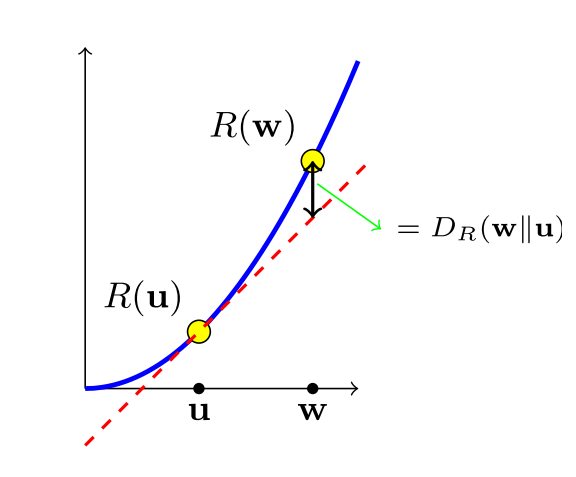
\includegraphics[width=1\textwidth]{./figures/bregman.png}
			\end{center}
		\end{column}
	\end{columns}	
	\begin{alertblock}{Regret Bound \scriptsize{ [Abernethy et al., COLT 2014]}}
		Assume that $\psi$ is  $\lambda-$ strongly convex with respect to $||.||$, $S$ is a closed convex set, and $||\mathbf{g}||_\star^2 \leq L$. OMD  with $\eta_t = \frac{C\sqrt{\lambda}}{\sqrt{\sum_{i = 1}^{t}||\mathbf{g}||_\star^2}}$ achieves:
		\begin{equation*}
			\mathrm{Regret}(\uu) \leq \frac{2CL}{\sqrt{\lambda}}\sqrt{T}.
		\end{equation*}		
	\end{alertblock}
\end{frame}

\begin{frame}
\frametitle{Converse Bounds }
\begin{block}{Lower Bounds \scriptsize{Classic Results: e.g. [Orabona, 2021]}}
	Let $S$ be any bounded convex set, $D = \mathrm{diam}(S)$, and $\mathcal{A}$ be any algorithm for Online Linear Optimization on $S$. There exists a sequence $\mathbf{g}_1, \dots, \mathbf{g}_T$ with $||\mathbf{g}_t||_2 \leq L$ such that
	\begin{equation*}
		\exists \uu \in S: \;\; \mathrm{Regret_T}(\uu) = \sum_{t = 1}^{T} \langle \w_t - \uu, \mathbf{g}_t\rangle  \geq \frac{\sqrt{2}LD\sqrt{T}}{4}.
	\end{equation*}
\end{block}
\end{frame}
	

\section{Relative Lipschitz Functions}
\framecard{\LARGE Relative Lipschitz Functions}
\begin{frame}{Relative Lipschitz Functions}
	\begin{exampleblock}{Definitions}
		A function $f: S \to \R$ is said to be \textbf{Lipschitz relative to  function $R$} if 
			\begin{equation*}
			\forall \x, \y \in S, \forall \mathbf{g} \in \partial f(\x):  ||\mathbf{g}||_*^2 \leq L^2 \frac{D_R(\y||\x)}{\frac{1}{2}||\y - \x||_2^2}
			\end{equation*}	
	\end{exampleblock}
	\begin{itemize}
		\item For example, the function $f(x) = x^2$ is not Lipschitz on $\mathbb{R}$. However, it is $f$ is $\sqrt{2}$-Lipschitz relative to $R(x) = 2x^4$.		
	\end{itemize}
\end{frame}


\section{Relative Lipschitz Functions in Online Learning}
\framecard{\LARGE Relative Lipschitz Functions\\ in Online Learning}
\begin{frame}
	\frametitle{Relative Lipschitzness in Online Learning}
		Relative Lipschitz Property was introduced in {\small [Lu et al., SIAM Opt., 2018]} for Convex Optimization.
	\begin{alertblock}{Relative Lipshitzness FTRL}
		If the functions $f_t$ is $L$-Lipschitz relative to $R$. 
		\begin{itemize}
			\item  \small [Zhou et al., NeurIPS, 2020]\\ The FTRL algorithm, $\w_{t+1} = \arg\min_{\w\in S} \big(\sum_{i = 1}^{t}f_t(\w) + \frac{1}{\eta_t}R(\w)\big)$,  achieves
			\vspace{-0.2cm}
			\begin{equation*}
			\mathrm{Regret}_T(\uu) \leq \frac{K}{\eta_T} + \sum_{t = 1}^{T} \frac{L^2 \eta_{t-1}}{2}.
			\end{equation*}
			
			\item  \small [B. M., 2020]\\ The FTRL algorithm, $\w_{t+1} = \arg\min_{\w\in S} \big(\sum_{i = 1}^{t}f_t(\w) + \frac{1}{\eta_t}\psi(\w)\big)$, achieves
			\vspace{-0.2cm}
			\begin{equation*}
			\mathrm{Regret}_T(\uu) \leq \frac{K}{\eta_T} + \sum_{t = 1}^{T} \frac{L^2 \eta_{t-1}}{2} + \sum_{t = 1}^{T} \frac{D_\epsilon(\x_{t+1}||\x_t)}{\eta_{t-1}}.
			\end{equation*}
			where $\epsilon(.) = R(.) - \psi(.)$.
		\end{itemize}
	\end{alertblock}
\end{frame}


\begin{frame}
	\frametitle{Relative Lipschitzness in Online Learning}	
	\begin{block}{Relative Lipshitzness OMD {\small [B. M., 2020]}}
		If the functions $f_t$ is $L$-Lipschitz relative to $R$, and we run Online Mirror Descent with $\eta_t$ and link function $\psi$, we have
		\begin{equation*}
			\mathrm{Regret}_T(\uu) = \frac{K}{\eta_T}+\sum_{t = 1}^{T} \frac{\eta_t L^2}{2} + \sum_{t = 1}^{T} \frac{D_\epsilon(\x_{t+1}||\x_{t})}{\eta_t},
		\end{equation*}
		where $\epsilon(.) = R(.) - \psi(.)$.
	\end{block}
\end{frame}

\begin{frame}
	\frametitle{Ongoing Work}	
	\begin{itemize}
		\item Online Convex Optimization with {\color{brown}Sub-Gaussian Noise}:
		\begin{itemize}
			\item The learner has access to a noisy version of the loss function or sub-gradient.
			\item How does the tail bound affect the Expected Regret?
			\item A similar problem was studied in \small{[Jun et al., COLT, 2019]} for Parameter-Free Online Learning.
		\end{itemize}
		\pause
		\vspace{0.1cm}
		
		\item {\color{brown}Parameter-Free} Online Learning with Relative Lipschitz Losses:
		\begin{itemize}
			\item Setting $\eta_t$ requires the knowledge of $L$ and $R$.
			\item Rich literature on parameter-free online learning:\\ {\small [Cutkosky, COLT 2020], [Orabona, NeurIPS, 2016].}
		\end{itemize}
		\pause
		\vspace{0.1cm}
		
		\item {\color{brown}Lower Bounds}: Classic techniques cannot be easily employed.
	\end{itemize}
\end{frame}


\section{Bibliography}
\framecard{\LARGE Bibliography}
\begin{frame}
	\frametitle{Bibliography}
	\begin{enumerate}
		\begin{scriptsize}
		\item F. Orabona.\\
		\textit{A Modern Introduction to Online Learning}.\\
		Monograph published in \textbf{ArXiv}, 2021.
		\item Y. Zhou, V. Portella, M. Schmidt, and N. Harvey.\\
		\textit{Regret Bounds without Lipschitz Continuity:
			Online Learning with Relative-Lipschitz Losses}.\\
		In \textbf{Neural Information Processing Systems (NeurIPS)}, 2020.			
		\item H. Lu, R. M. Freund, and Y. Nesterov.\\
		\textit{Relatively smooth convex optimization by first-order methods and applications}.\\
		In \textbf{SIAM Journal on Optimization}, 28(1):333-354, 2018.
		\item K. Jun and F. Orabona\\
		\textit{Parameter-Free Online Convex Optimization with Sub-Exponential Noise}.\\
		In \textbf{Conference on Learning Theory (COLT)}, 2019.
		\item F. Orabona, D, P\'al.\\
		\textit{Coin Betting and Parameter-Free Online Learning}.\\
		In \textbf{Neural Information Processing Systems (NeurIPS)}, 2016.			
		\item A. Cutkosky.\\
		\textit{Artificial Constraints and Lipschitz Hints for Unconstrained Online Learning}.\\\vspace{-0.1cm}
		In \textbf{Conference on Learning Theory (COLT)}, 2020.					
		\end{scriptsize}
	\end{enumerate}
\end{frame}


\end{document}